\chapter{Implementazione di BERTopic}

\section{Embedding}
I modelli principali consigliati nella documentazione\footnote{\url{https://maartengr.github.io/BERTopic/getting_started/embeddings/embeddings.html}} sono i \textbf{sentence transformers} (SBERT).
Ci sono molti modelli SBERT pre-addestrati tra cui scegliere, la documentazione ufficiale nei suoi esempi usa spesso all-MiniLM-L6-v2 un modello estremamente leggero e veloce, però non sufficientemente preciso nel catturare sfumature semantiche complesse o relazioni a lungo raggio.
paraphrase-MiniLM-L12-v2 e paraphrase-mpnet-base-v2, sono più accurati, ma più specializzati nel catturare relazioni di parafrasi, fra testi molto simili, sono inoltre inadatti a testi particolarmente lunghi come gli annunci di lavoro.
\textbf{all-mpnet-base-v2}, invece, ha una alta \textbf{precisione semantica}, e si comporta bene con documenti di lunghezza \textbf{medio-lunga}.
Ha però un limite di lunghezza di \textbf{512 token}.
Ecco alcune informazioni sulla lunghezza del nostro dataset (dopo la pulizia):
\begin{figure}[H]
\centering
\scriptsize
\begin{tabular}{lccc}
\hline
 & n chars & n words & n tokens mpnet \\
\hline
count & 5357.00 & 5357.00 & 5357.00 \\
mean & 3315.48 & 457.92 & 594.54 \\
std & 1591.28 & 219.01 & 283.37 \\
min & 91.00 & 14.00 & 23.00 \\
50\% & 3087.00 & 427.00 & 554.00 \\
75\% & 4060.00 & 562.00 & 729.00 \\
90\% & 5213.40 & 717.00 & 934.00 \\
95\% & 6188.20 & 846.20 & 1103.40 \\
99\% & 8797.52 & 1203.44 & 1562.72 \\
max & 19470.00 & 2739.00 & 3753.00 \\
\hline
\multicolumn{4}{l}{Testi che superano i 512 token: 3075 (57.40\%)} \\
\multicolumn{4}{l}{Totale annunci: 5357} \\
\hline
\end{tabular}
\caption{Statistiche globali del dataset (totale annunci: 5357).}
\label{fig:dataset-stats}
\end{figure}
\noindent Quando SBERT riceve un input troppo lungo, lo \textbf{tronca} questo significa che applicando l'embedder così come è verrebbe tagliata una porzione molto grande del dataset.

\noindent Le prime opzioni che abbiamo considerato sono:
\begin{enumerate}
    \item Affidarsi ad un modello con un limite di dimensione input più alto (ad esempio \textbf{all-roberta-long-v1})
    \item Frammentare le descrizioni e fare il topic modeling in segmenti di quest'ultime.
\end{enumerate}
Il vantaggio della prima opzione è che i modelli \textit{long-context}, mantengono attenzione tra termini distanti, permettendo di cogliere relazioni semantiche a lungo raggio, cosa impossibile se si divide il testo in \textit{chunk}.
Non è però una caratteristica che abbiamo ritenuto significativa, data la natura del nostro \textit{dataset}, infatti i nostri paragrafi hanno natura scollegata, uno potrebbe parlare di competenze e un altro di mansioni, la coerenza globale è più importante in testi di natura \textbf{discorsiva}.
Inoltre se la lunghezza del testo è grande è probabile che contenga più temi, un unico embedding rischia di mescolare \textbf{sezioni semanticamente diverse}, ottenendo topic più grossolani.
La seconda opzione invece, oltre che generare topic più \textbf{puliti} e \textbf{interpretabili}, consente di aumentare molto il numero di documenti in input e questo è un vantaggio per dataset esegui come il nostro.
Però anche questo caso presenta delle criticità: non avremmo i topic relativi agli annunci come uniche entità, ma saranno relativi ai segmenti e andrebbero aggregati a posteriori per ottenere una \textbf{distribuzione di topic per annuncio}. In più in questo modo, gli annunci più lunghi avranno \textbf{più peso}, semplicemente perché hanno più paragrafi. La situazione si complica ulteriormente se i documenti contengono paragrafi simili, questo creerebbe dei \textbf{cluster} artefatti e quindi topic che non rispecchiano la natura del dataset. Un altro problema è che con questo metodo il modello è completamente ignaro della struttura globale dell'annuncio.
Questo approccio è più attuabile per risolvere un problema di \textbf{classificazione}, non per il \textit{topic modeling}.\medskip

\noindent La soluzione che abbiamo scelto è dunque quella di \textit{mean-max-pooling}.
\subsection{Mean-max pooling}

\noindent Con questa tecnica si ottiene un embedding per ogni annuncio partendo dagli embedding dei paragrafi, seguendo i passaggi seguenti:
\begin{enumerate}
    \item calcolare gli embedding di ciascun paragrafo;
    \item normalizzare ogni embedding;
    \item calcolare media aritmetica e massimo elemento per elemento;
    \item concatenare i due vettori risultanti;
    \item normalizzare nuovamente il vettore concatenato.
\end{enumerate}

In questo modo si ottiene un embedding unico di dimensione doppia rispetto l'output dell'embedder che può catturare sia il \textbf{significato generale} dell'annuncio, sia le \textbf{feature salienti} dei singoli paragrafi: queste due componenti possono produrre vettori più \textbf{discriminativi} e quindi più facilmente separabili nello spazio semantico.

Per attuare questo approccio serve inoltre una strategia di segmentazione degli annunci che soddisfi al contempo \textbf{coerenza semantica} e criteri di lunghezza: il segmento non può essere troppo corto, altrimenti SBERT non ha il contesto per estrarre topic singnificativi, e non può ovviamente superare la lunghezza massima consentita. Approfondiamo questo aspetto nel capitolo \textbf{Pre-processing}.

\section{Dimensionality Reduction}
Si osservi come per valori ridotti di \texttt{n\_neighbors} la proiezione UMAP mantenga dettagli locali (curve delle zanne o delle zampe), ma perda la forma complessiva del mammut; all'aumentare del parametro la sagoma globale diventa riconoscibile, a scapito delle piccole variazioni geometriche. In modo analogo, sperimentare con valori come 15, 50 o 100 nel nostro dataset permette di calibrare il livello di granularità dei topic: valori molto bassi frammentano in gruppi minuti, mentre impostazioni alte tendono a fondere i cluster semantici più affini; una scelta intermedia (ad esempio \texttt{n\_neighbors} = 50) offre un equilibrio adeguato tra dettaglio locale e coerenza globale.

Per giungere a questa scelta sono stati provati diversi set di iperparametri; riportiamo di seguito quelli usati per la configurazione finale, così da facilitarne la riproducibilità:

\begin{lstlisting}[language=Python]
umap_model = UMAP(
    n_neighbors=n,
    n_components=10,
    min_dist=0.0,
    metric="cosine",
    random_state=1,
)
hdbscan_model = HDBSCAN(
    min_cluster_size=50,
    min_samples=15,
    metric="euclidean",
    cluster_selection_method="eom",
    prediction_data=True,
    cluster_selection_epsilon=0.1,
)
\end{lstlisting}

\begin{table}[H]
\centering
\footnotesize
\begin{tabular}{rrrrrr}
\hline
$n\_neighbors$ & $n\_topics$ & mean cluster size & std cluster size & topics $<100$ & topics $>500$ \\
\hline
15  & 15 & 208.87 & 267.01 & 8  & 2 \\
50  & 61 & 224.98 & 294.64 & 25 & 8 \\
60  & 62 & 197.81 & 254.00 & 26 & 6 \\
70  & 58 & 208.09 & 242.64 & 22 & 4 \\
100 & 2  & 2396.50 & 2090.91 & 0  & 2 \\
\hline
\end{tabular}
\caption{Sintesi degli esperimenti al variare di $n\_neighbors$: numero di topic trovati, dimensione media e deviazione standard dei cluster, oltre al conteggio dei topic piccoli ($<100$ documenti) e molto grandi ($>500$ documenti).}
\label{tab:n-neighbors-summary}
\end{table}

\noindent Nel corso dei test abbiamo variato \texttt{n\_neighbors} tra i valori 15, 50, 60 e 70 (con un confronto a 100 come baseline), scegliendo infine \texttt{n\_neighbors} = 50 come compromesso ottimale; la Tabella~\ref{tab:n-neighbors-summary} riassume il numero di topic e la distribuzione delle dimensioni dei cluster ottenuti in ciascun caso.

\begin{figure}[H]
\centering
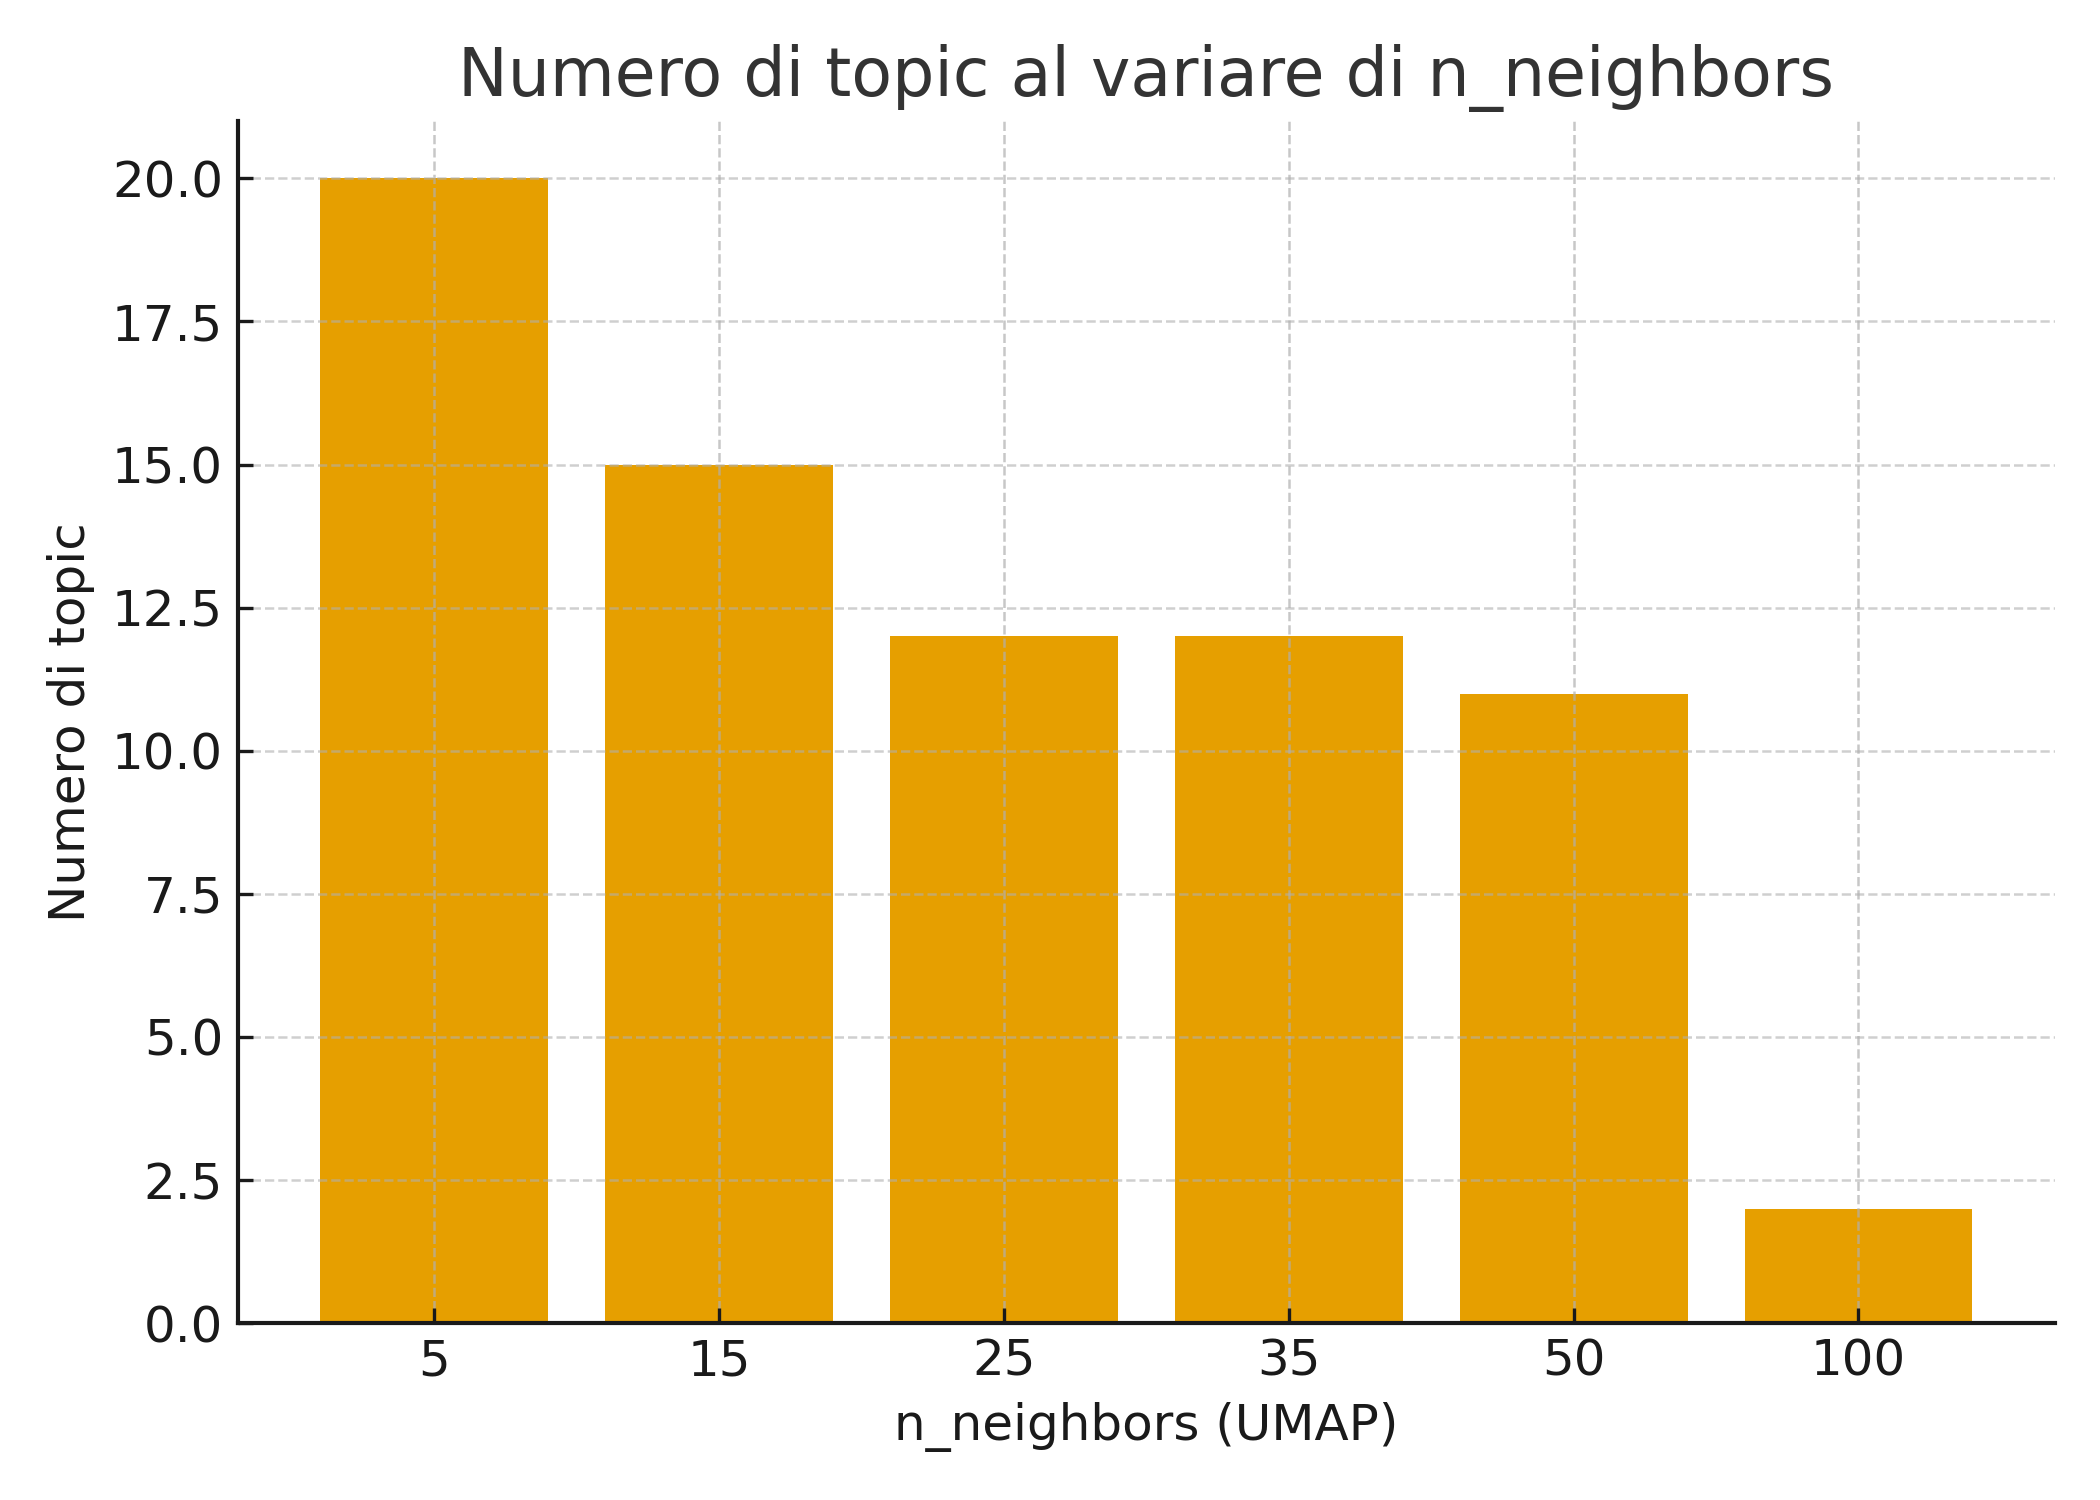
\includegraphics[width=0.6\textwidth]{BERTopic/umap/num_topics_per_neighbors.png}
\caption{Numero di topic generati da HDBSCAN al variare di $n\_neighbors$: la scelta intermedia ($n\_neighbors=50$) massimizza la granularità senza collassare in pochi cluster.}
\label{fig:num-topics-per-neighbors}
\end{figure}
\noindent I plot in Figura~\ref{fig:umap-neighbors-comparison} mostrano la proiezione bidimensionale generata da \texttt{BERTopic.\allowbreak visualize\_documents()} per tre configurazioni distinte. Con \texttt{n\_neighbors} = 15 UMAP costruisce un grafo molto \textbf{frammentato}: le connessioni tra i documenti sono deboli, molti punti rimangono isolati e HDBSCAN li etichetta come \textit{outlier}, generando quindi un topic \texttt{-1} (il topic dove vengono inseriti i documenti di cui si è incerti) estremamente popoloso (2224 documenti). All'estremo opposto (\texttt{n\_neighbors} = 100) il grafo è troppo \textbf{compatto}: le relazioni globali dominano e i topic tendono a fondersi. Con \texttt{n\_neighbors} = 50, invece, i cluster si addensano in regioni coerenti, evidenziando macro-categorie professionali distinte (marketing, cybersecurity, biomedical engineering, \emph{etc.}). L'incrocio tra indicatori numerici e analisi visiva conferma quindi \texttt{n\_neighbors} = 50 come valore finale.

\begin{figure}[H]
\centering
\begin{subfigure}{0.32\textwidth}
    \centering
    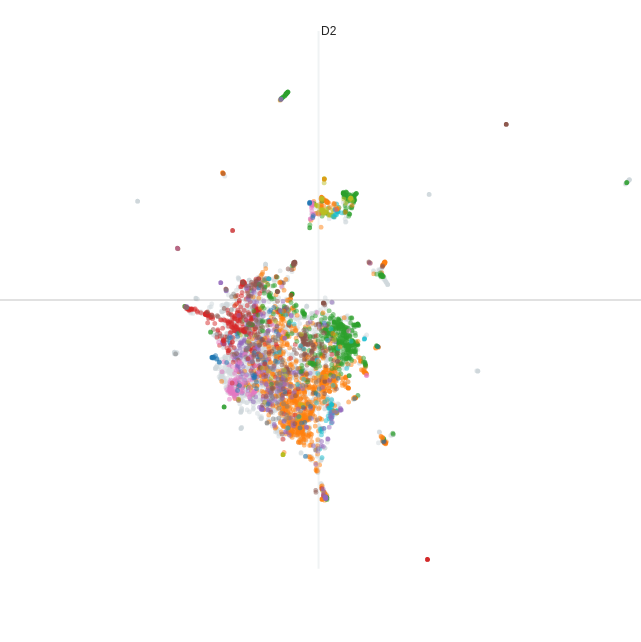
\includegraphics[width=\textwidth]{BERTopic/umap/umap_15.png}
    \caption{$n\_neighbors = 15$}
\end{subfigure}\hfill
\begin{subfigure}{0.32\textwidth}
    \centering
    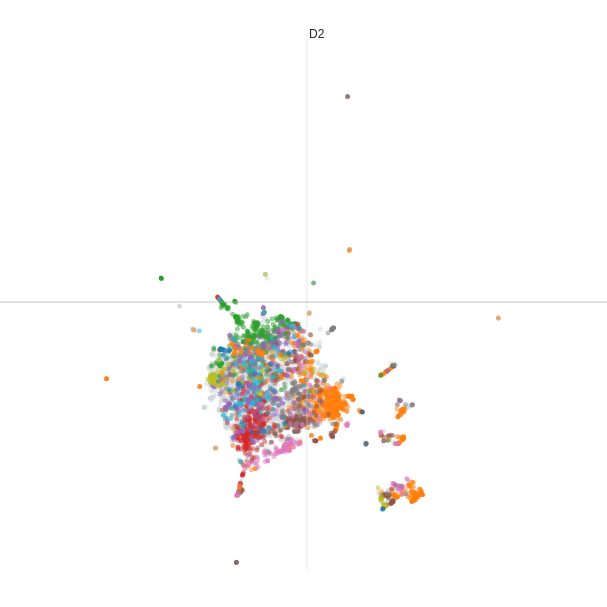
\includegraphics[width=\textwidth]{BERTopic/umap/umap_50.png}
    \caption{$n\_neighbors = 50$}
\end{subfigure}\hfill
\begin{subfigure}{0.32\textwidth}
    \centering
    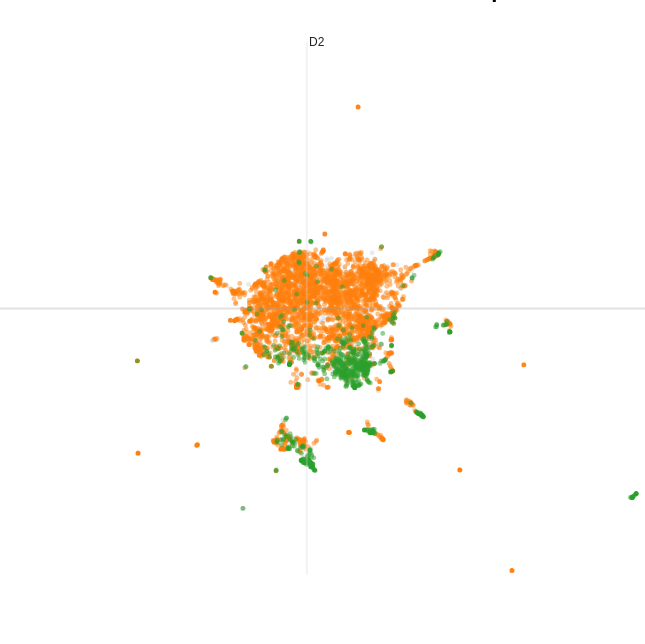
\includegraphics[width=\textwidth]{BERTopic/umap/umap_100.png}
    \caption{$n\_neighbors = 100$}
\end{subfigure}
\caption{Proiezioni generate da \texttt{BERTopic.\allowbreak visualize\_documents()}: i punti (embedding ridotti a 2 dimensioni) sono colorati in base al topic. Confronto tra \texttt{n\_neighbors} pari a 15, 50 e 100.}
\label{fig:umap-neighbors-comparison}
\end{figure}

\noindent Abbiamo fissato \texttt{min\_dist} a $0.0$ poiché l'algoritmo di \emph{clustering} (HDBSCAN) restituisce risultati migliori con cluster densi e ben separati: eventuali regioni vuote verrebbero classificate come outlier e assegnate al topic ``spazzatura'' (\texttt{-1}). Mantenere gli embedding compatti riduce la formazione di tali zone.

\section{Clustering}
Abbiamo però introdotto un parametro \texttt{min\_samples}: al suo crescere aumenta la \texttt{core\_distance} media e con essa i punti considerati rarefatti.
Quindi più è alto \texttt{min\_samples}, più embedding verranno considerati come \textit{rumore}.
Come per \texttt{n\_neighbors}, mostriamo qui dei confronti con diversi valori di \texttt{min\_samples}:

\begin{table}[H]
\centering
\footnotesize
\begin{tabular}{lrrrrrrr}
\hline
min\_samples & n\_topics & noise \% & mean size & median size & max size & top topic \% & outliers \\
\hline
5  & 12 & 42.28 & 257.67 & 190.0 & 882  & 28.53  & 2265 \\
15 & 61 & 45.88 & 224.98 & 131.0 & 1581 & 11.52 & 11635 \\
30 & 10 & 39.69 & 323.10 & 209.0 & 886  & 27.42  & 2126 \\
60 & 2  & 14.80 & 2282.00 & 2282.0 & 3699 & 81.05  & 793  \\
\hline
\end{tabular}
\caption{Metriche chiave al variare di \texttt{min\_samples}: numero di topic (n\_topics), percentuale di rumore (noise), statistiche di dimensione dei cluster, quota del topic principale e conteggio degli outlier.}
\label{tab:min-samples-summary}
\end{table}
Per valori molto bassi (\texttt{min\_samples} = 5) l'algoritmo tende a frammentare eccessivamente il corpus, generando numerosi micro-cluster spesso composti da pochi paragrafi. 
Sebbene questa impostazione aumenti il livello di dettaglio, i topic risultano meno stabili e semanticamente meno coerenti.

Aumentando il parametro a valori intermedi (\texttt{min\_samples} = 15) si ottiene un equilibrio tra granularità e stabilità. 
I cluster formati risultano sufficientemente omogenei e interpretabili, mantenendo al contempo un numero di topic adeguato per una lettura tematica fine del corpus. 
Questo valore rappresenta il compromesso ottimale tra dettaglio informativo e robustezza del clustering.

Con valori più elevati (\texttt{min\_samples} = 30) l’algoritmo diventa più selettivo: la quantità di rumore aumenta e alcuni cluster tendono a fondersi, riducendo la capacità di distinguere tematiche affini ma distinte. 
Spingendosi ulteriormente verso valori molto alti (\texttt{min\_samples} = 60) si osserva un drastico calo del numero di cluster e un incremento marcato dei punti etichettati come rumore, con il rischio di ottenere pochi macro-temi troppo generici.

\begin{figure}[H]
\centering
\begin{subfigure}{0.24\textwidth}
    \centering
    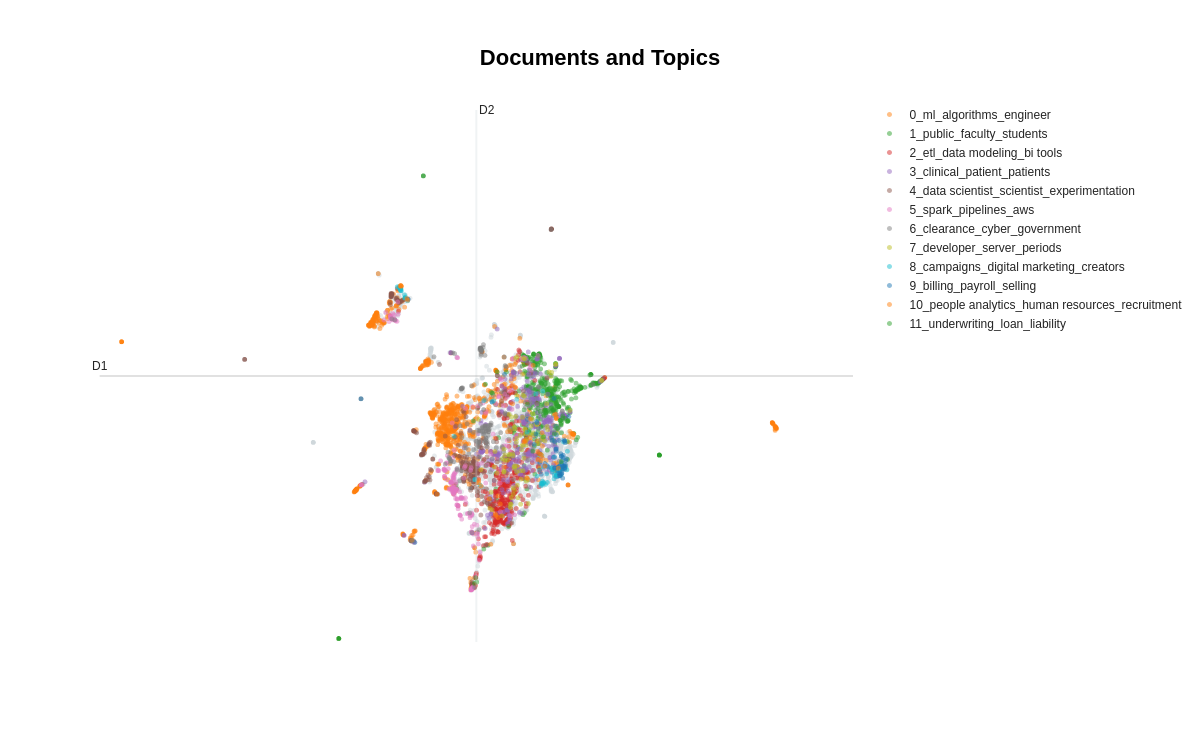
\includegraphics[width=\textwidth]{BERTopic/hdbscan/ms5.png}
    \caption{\texttt{min\_samples} = 5}
\end{subfigure}\hfill
\begin{subfigure}{0.24\textwidth}
    \centering
    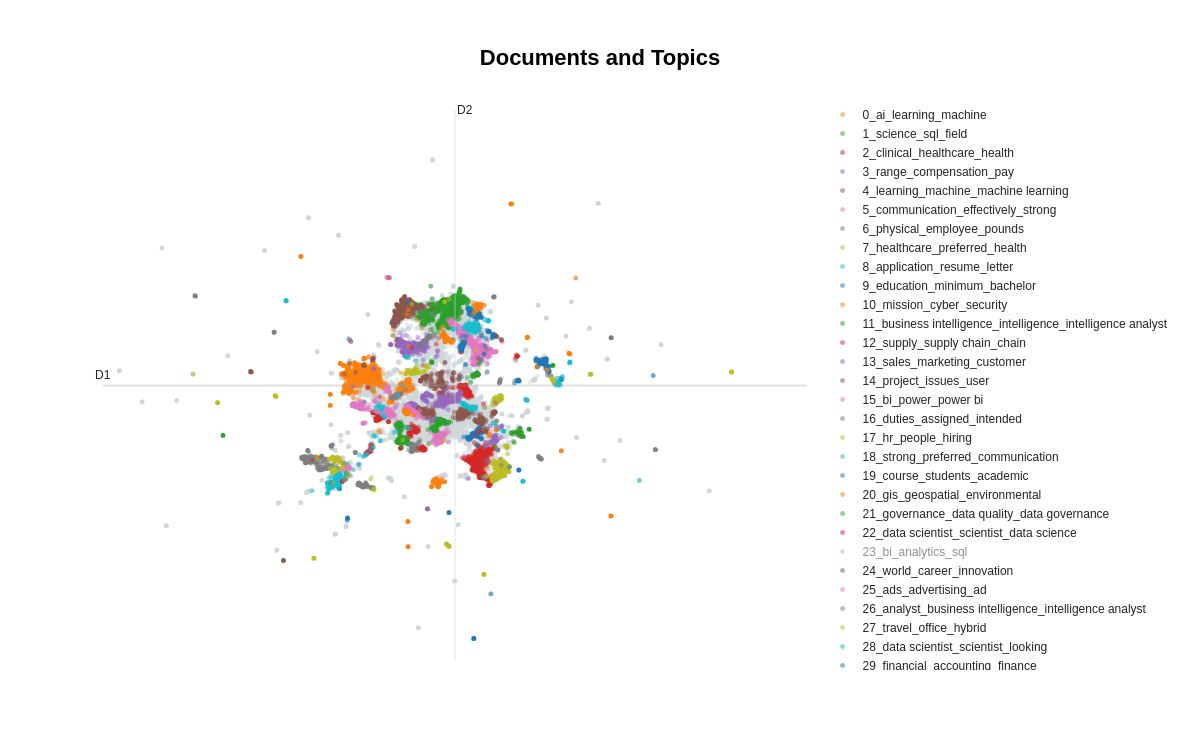
\includegraphics[width=\textwidth]{BERTopic/hdbscan/ms15.png}
    \caption{\texttt{min\_samples} = 15}
\end{subfigure}\hfill
\begin{subfigure}{0.24\textwidth}
    \centering
    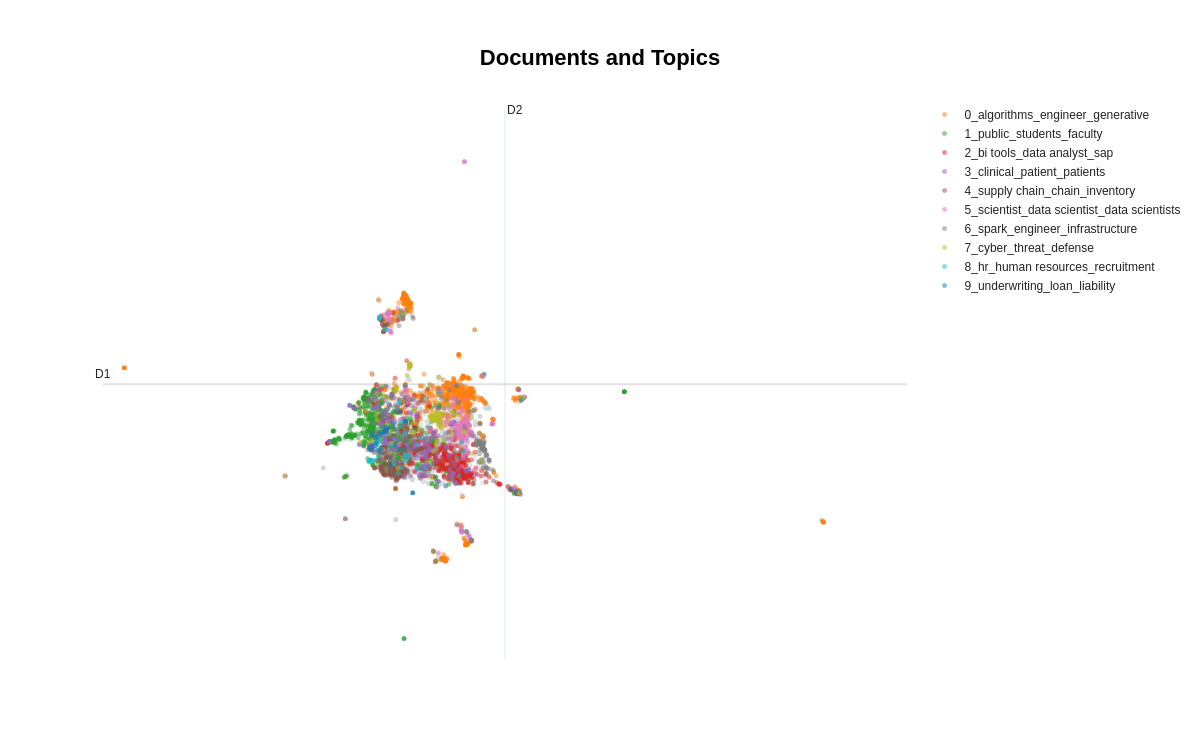
\includegraphics[width=\textwidth]{BERTopic/hdbscan/ms30.png}
    \caption{\texttt{min\_samples} = 30}
\end{subfigure}\hfill
\begin{subfigure}{0.24\textwidth}
    \centering
    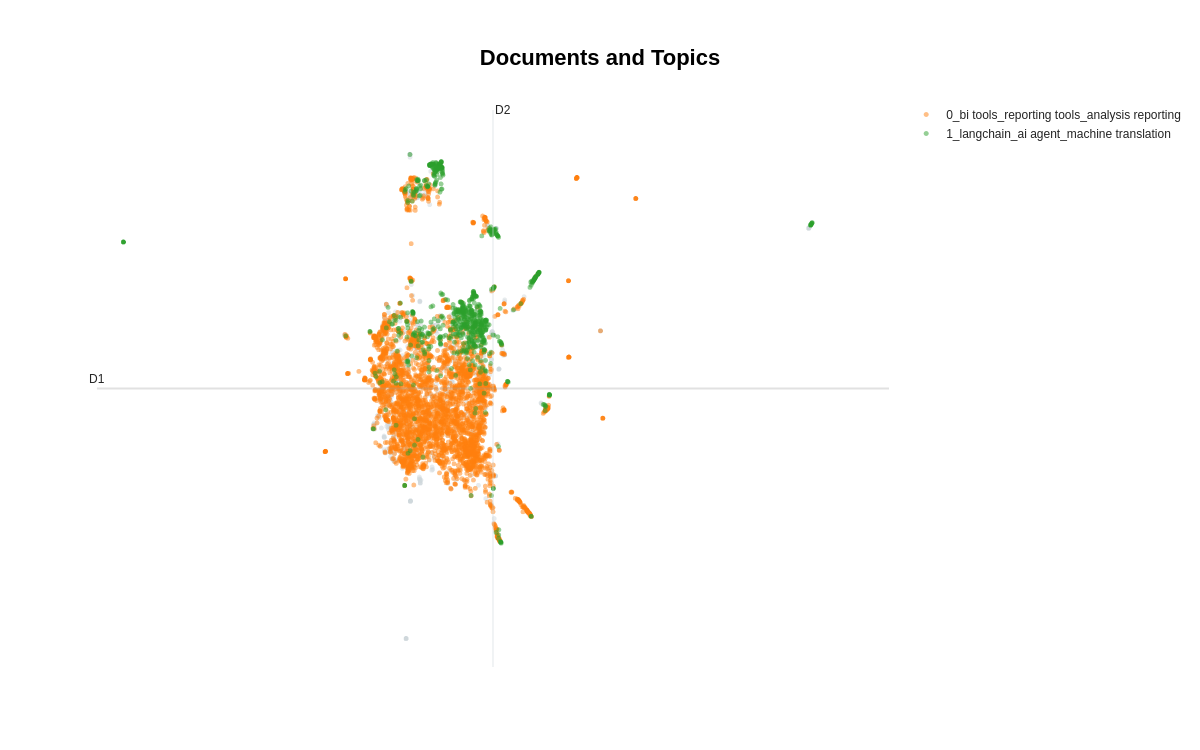
\includegraphics[width=\textwidth]{BERTopic/hdbscan/ms_60.png}
    \caption{\texttt{min\_samples} = 60}
\end{subfigure}
\caption{Effetto di \texttt{min\_samples} sulla distribuzione dei topic: visualizzazioni prodotte da \texttt{BERTopic.visualize\_documents()} in configurazioni crescenti del parametro.}
\label{fig:min-samples-umap}
\end{figure}

Nel complesso, la configurazione con \texttt{min\_samples} = 15 si è dimostrata la più bilanciata: 
garantisce la formazione di cluster stabili, coerenti e sufficientemente dettagliati, risultando quindi la scelta più appropriata per il corpus di annunci di lavoro considerato.
